\documentclass{article}
\usepackage{geometry}
 \geometry{
 a4paper,
 total={170mm,257mm},
 left=20mm,
 top=20mm,
 }
\usepackage[english,greek, main=greek]{babel}
\usepackage[utf8]{inputenc}
\usepackage{amsmath}
\usepackage{graphicx} % for graphics and plots
\usepackage{subcaption} % for subfigures and subcaptions and \ContinuedFloat
\usepackage{placeins} % for \FloatBarrier
\usepackage{xcolor} % for colour definitions
\usepackage{listings} % for code highlighting
\usepackage{verbatim} % for file input
\usepackage{varwidth} % for centering verbatim 
\usepackage{hyperref} % clickable links
\usepackage{datatool} % for csv reading
\usepackage{tikz} % for tikz plot
\usepackage{adjustbox} % for table scaling
\usepackage{pmboxdraw} % for box drawing characters
\usetikzlibrary{datavisualization, babel} % for tikz plots
\usepackage{fancyvrb} % for haskell code
\DefineVerbatimEnvironment{code}{Verbatim}{fontsize=\small}
\DefineVerbatimEnvironment{example}{Verbatim}{fontsize=\small}
\newcommand{\ignore}[1]{}
\newcommand{\eng}[1]{\foreignlanguage{english}{#1}} % shortcut for inserting english into greek text

\useshorthands{;}
\defineshorthand{;}{?} % greek question mark instead of english semicolon

\lstset{
  frame=none,
  xleftmargin=2pt,
  stepnumber=1,
  numbers=left,
  numbersep=5pt,
  numberstyle=\ttfamily\tiny\color[gray]{0.3},
  belowcaptionskip=\bigskipamount,
  captionpos=b,
  escapeinside={*'}{'*},
  language=haskell,
  tabsize=2,
  emphstyle={\bf},
  commentstyle=\it,
  stringstyle=\mdseries\rmfamily,
  showspaces=false,
  keywordstyle=\bfseries\rmfamily,
  columns=flexible,
  basicstyle=\small\sffamily,
  showstringspaces=false,
  morecomment=[l]\%,
  xleftmargin=.2\textwidth, xrightmargin=.2\textwidth
}

\title{
    \includegraphics[width=\textwidth]{~/Pictures/emp.png} \\
    \vskip 5cm
    Κατανεμημένα Συστήματα \\
    \large Εξαμηνιαία Εργασία - \eng{BlockChat} 
    \vskip 5cm
}

\author{ Αναστάσιος Στέφανος Αναγνώστου \\ \large 03119051 }

\begin{document}

\maketitle \clearpage \tableofcontents \clearpage

\part{Σχεδιασμός Συστήματος}

Αρχικά, ο κώδικας αποτελείται από τα παρακάτω αρχεία με την δομή που φαίνεται:

\begin{figure}[ht]
    \centering
    \selectlanguage{english}
    \begin{varwidth}{\linewidth}
        \verbatiminput{project-structure.txt}
    \end{varwidth}
    \selectlanguage{greek}
    \caption{Δομή του κώδικα}
\end{figure}

Το αρχείο \texttt{\eng{Main.hs}} είναι ο οδηγός της εφαρμογής, δηλαδή αυτό που
εκτελείται για την εκκίνηση του προγράμματος. Στο αρχείο \texttt{\eng{CLI.hs}}
υλοποιείται το \eng{front-end} της εφαρμογής, δηλαδή η διεπαφή με τον χρήστη.
Τα υπόλοιπα αρχεία είναι το \texttt{\eng{back-end}} της εφαρμογής, δηλαδή οι απαραίτητες
συναρτήσεις και η λογική για την λειτουργία του \eng{blockchain} δικτύου. Εξαίρεση
αποτελούν τα αρχεία \texttt{\eng{Utils.hs}} και \texttt{\eng{Types.hs}} τα οποία
περιέχουν βοηθητικές συναρτήσεις και δηλώσεις τύπους δεδομένων αντίστοιχα.

\section{\eng{Back-end}}

\subsection{Βασικές Δομές Δεδομένων}

Αρχικά θα αναλυθούν οι βασικές δομές δεδομένων που χρησιμοποιούνται στο
σύστημα. Αυτές είναι:

\selectlanguage{english}
\begin{itemize}
    \item Wallet
    \item Account
    \item Block
    \item Transaction
\end{itemize}
\selectlanguage{greek}

\subsubsection{\eng{Wallet}}

Το αρχείο \texttt{\eng{Wallet.hs}} περιέχει την υλοποίηση της δομής \eng{Wallet}.
Ορίζει για τα υπόλοιπα αρχεία τον τύπο \texttt{\eng{Wallet}}, ως ένα συνώνυμο
για ένα ζευγάρι από \texttt{\eng{PublicKey, PrivateKey}} και την συνάρτηση
\texttt{\eng{generateWallet}}, η οποία δημιουργεί ένα τέτοιο ζευγάρι κλειδιών.

\begin{figure}[ht]
\selectlanguage{english}
    \lstinputlisting[label={walleths}, caption={Wallet.hs}, language={haskell}]{../src/Wallet.hs}
\selectlanguage{greek}
\end{figure}
\FloatBarrier

\subsubsection{\eng{Account}}

Το αρχείο \texttt{\eng{Account.hs}} περιέχει την υλοποίηση της δομής \eng{Account}.
Ορίζει για τα υπόλοιπα αρχεία των τύπο, καθώς και πρόσβαση σε όλα τα πεδία του,
μία μεταβλητή (βασικά, σταθερή συνάρτηση) \texttt{\eng{initialAccount}} και κάποιες
βοηθητικές συναρτήσεις για την ενημέρωση του λογαριασμού και γρήγορη πρόσβαση στο
υπόλοιπό του, λαμβάνοντας υπόψιν το \eng{staking}. Δύο πράγματα είναι αξιοσημείωτα
σε αυτό το σημείο:

\begin{enumerate}
    \item Η σταθερή συνάρτηση / μεταβλητή \texttt{\eng{initialAccount}} χρησιμοποιείται
        από τους κόμβους για την αρχικοποίηση του λογαριασμού τους. Αυτό σημαίνει ότι
        ο \eng{bootstrap} κόμβος δεν χρειάζεται να τους στείλει κάποια αρχική πληροφορία
        σχετική με τον λογαριασμό τους.
    \item Η συνάρτηση \texttt{\eng{updateStake}} πανωγράφει το προηγούμενο ποσό
        \eng{stake}. Αυτό επιτρέπει στον χρήστη της εφαρμογής να ενημερώνει το
        \eng{stake} του.
\end{enumerate}

\selectlanguage{english}
    \lstinputlisting[firstline=11, label={accounths}, caption={Account.hs}, language={haskell}]{../src/Account.hs}
\selectlanguage{greek}

\subsubsection{\eng{Block}}

Το αρχείο για τον ορισμό της δομής \texttt{\eng{Block}} θα αναλυθεί σε τμήματα, καθώς
εμπεριέχει διάφορα μέρη τα οποία εξυπηρετούν ανεξάρτητους μεταξύ τους σκοπούς.

Αρχικά, στο \ref{lst:blockhs1} φαίνεται, εκτός από κάποιες απαραίτητες εισαγωγές βιβλιοθηκών,
η δήλωση της δομής \texttt{\eng{BlockInit}}. Αυτή η δομή χρησιμοποιείται ως βοηθητική δομή
για την κανονική δομή \texttt{\eng{Block}}. Εμπεριέχει όλα τα πεδία του \eng{block} εκτός
από το \eng{hash}, το οποίο υπολογίζεται και συμπεριλαμβάνεται κατά την δημιουργία ενός
στιγμιοτύπου της δομής \texttt{\eng{Block}}. 

    \selectlanguage{english}
    \lstinputlisting[firstline=29, lastline=35,label={lst:blockhs1}, caption={Block.hs}, language={haskell}]{../src/Block.hs}
    \selectlanguage{greek}

Στην συνέχεια, το \texttt{\eng{BlockInit}} ορίζεται ως στιγμιότυπο της κατηγορίας κλάσεων
\texttt{\eng{Binary}}, ώστε να μπορεί να κωδικοποιηθεί σε \eng{bytes} προς αποστολή και προς
\eng{hash}άρισμα.

    \selectlanguage{english}
    \lstinputlisting[firstline=37, lastline=51,label={lst:blockhs2}, caption=Block.hs, language=haskell]{../src/Block.hs}
    \selectlanguage{greek}

Στην συνέχεια \ref{lst:blockhs3}, ορίζεται η δομή \texttt{\eng{Block}}, η οποία
περιέχει ακόμα το πεδίο \texttt{\eng{blockCurrentHash}}. Ορίζεται και αυτή ως
στιγμιότυπο της κατηγορίας κλάσεων \texttt{\eng{Binary}} για τους ίδιους λόγους
με το \texttt{\eng{BlockInit}}.

    \selectlanguage{english}
    \lstinputlisting[firstline=53, lastline=79,label={lst:blockhs3}, caption=Block.hs, language=haskell]{../src/Block.hs}
    \selectlanguage{greek}

Ακόμα, στο \ref{lst:blockhs4} ορίζεται η συνάρτηση \texttt{\eng{computeHash}} η οποία
συμπληρώνει το πεδίο \texttt{\eng{blockCurrentHash}} του \texttt{\eng{Block}} δεδομένου
ενός \texttt{\eng{BlockInit}}, ορίζεται η \texttt{\eng{finalizeBlock}}, η οποία 
επιστρέφει ένα ολοκληρωμένο \texttt{\eng{Block}} από ένα \texttt{\eng{BlockInit}} και
τέλος η \texttt{\eng{createBlock}} η οποία είναι ένα \eng{wrapper} για την
\texttt{\eng{finalizeBlock}} και προσφέρεται στον υπόλοιπο κώδικα ως η μέθοδος
για την δημιουργία ενός \texttt{\eng{Block}}.

    \selectlanguage{english}
    \lstinputlisting[firstline=84, lastline=101,label={lst:blockhs4}, caption=Block.hs, language=haskell]{../src/Block.hs}
    \selectlanguage{greek}

Εδώ ορίζεται ένα συνώνυμο τύπου και μία βοηθητική σταθερά.

    \selectlanguage{english}
    \lstinputlisting[firstline=103, lastline=107,label={lst:blockhs5}, caption=Block.hs, language=haskell]{../src/Block.hs}
    \selectlanguage{greek}

Τέλος, ορίζονται συναρτήσεις για την αποστολή ενός \eng{Block} στο δίκτυο και την
επικύρωση ενός \eng{Block}. Ακόμα, ορίζονται κάποιες βοηθητικές συναρτήσεις για τον
υπολογισμό του μέσου \eng{block time} από τα \eng{time stamps} των \eng{Block} στην
αλυσίδα.
% consider a figure environment
    \selectlanguage{english}
    \lstinputlisting[firstline=109, lastline=139,label={lst:blockhs6}, caption=Block.hs, language=haskell]{../src/Block.hs}
    \selectlanguage{greek}
\FloatBarrier

\subsubsection{\eng{Transaction}}

Ο κώδικας για την υλοποίηση της δομής \eng{Transaction} ακολουθεί τις ίδιες αρχές με
τον κώδικα για την υλοποίηση της δομής \eng{Block}. Για αυτόν τον λόγο δεν θα παρουσιαστεί
ολόκληρος αλλά τα πιο σημαντικά μέρη.

Αρχικά, και αυτός ο τύπος ορίζεται ως στιγμιότυπο της κατηγορίας κλάσεων \eng{Binary}, επειδή
πρέπει και αυτός να μπορεί να κωδικοποιηθεί σε \eng{bytes} για την αποστολή του στο δίκτυο.

Οι πιο σημαντικές συναρτήσεις είναι οι ακόλουθες:

\begin{figure}[ht]
    \selectlanguage{english}
    \lstinputlisting[firstline=169, label={lst:transactionhs1}, caption=Transaction.hs, language=haskell]{../src/Transaction.hs}
    \selectlanguage{greek}
\end{figure}
\FloatBarrier

όπου \texttt{\eng{PubKeyToAcc}} και \texttt{\eng{Peer}} είναι τύποι που ορίζονται στο
αρχείο \texttt{\eng{Types.hs}}:

\begin{figure}[ht]
    \selectlanguage{english}
    \lstinputlisting[firstline=11, label={lst:typeshs}, caption=Types.hs, language=haskell]{../src/Types.hs}
    \selectlanguage{greek}
\end{figure}
\FloatBarrier

ενώ η συνάρτηση \texttt{\eng{encodeStrict}} ορίζεται στο αρχείο \texttt{\eng{Utils.hs}}:

    \selectlanguage{english}
    \lstinputlisting[firstline=14, label={lst:utilshs}, caption=Utils.hs, language=haskell]{../src/Utils.hs}
    \selectlanguage{greek}

Σημαντική επίσης είναι η ακόλουθη συνάρτηση, που χρησιμοποιείται για την ενημέρωση των
λογαριασμών βάσει μίας συναλλαγής, και η επέκτασή της σε λίστα συναλλαγών. Αυτές θα
χρησιμοποιηθούν από τους κόμβους για την ενημέρωση του \eng{soft state} τους.
Παρατηρείται ότι δεν ενημερώνουν το \eng{nonce} του λογαριασμού. Για πρακτικούς
λόγους, που μπορούν να εξηγηθούν αναλυτικά αργότερα, στον κώδικα των κόμβων,
η ενημέρωση γίνεται από το \eng{front-end}.

    \selectlanguage{english}
    \lstinputlisting[firstline=112, lastline=141, label={lst:transactionhs2}, caption=Transaction.hs, language=haskell]{../src/Transaction.hs}
    \selectlanguage{greek}

Τέλος, φαίνεται η συνάρτηση \texttt{\eng{createTransaction}} που θα χρησιμοποιείται
για την δημιουργία συναλλαγών και κάποιες βοηθητικές συναρτήσεις, ίδιες στην λογική
και στην δομή με τις αντίστοιχες του \texttt{\eng{Block.hs}}.

% consider a figure environment
\selectlanguage{english}
\lstinputlisting[firstline=143, lastline=167, label={lst:transactionhs3}, caption=Transaction.hs, language=haskell]{../src/Transaction.hs}
\selectlanguage{greek}

\subsection{Κόμβοι}

Η λογική των κόμβων διατυπώνεται στα αρχεία \texttt{\eng{OrdinaryNode.hs}} και
\texttt{\eng{BootstrapNode.hs}}. Στο πρώτο αρχείο ορίζεται η λογική των κόμβων
που συμμετέχουν στο δίκτυο, ενώ στο δεύτερο ορίζεται η λογική του κόμβου που
είναι υπεύθυνος για την αρχικοποίηση του δικτύου.

\subsubsection{\eng{BootstrapNode}}

Κατ'αρχάς, ορίζονται κάποιοι βοηθητικοί τύποι:

    \selectlanguage{english}
    \lstinputlisting[firstline=51, lastline=79, label={lst:bootstrapnodehs1}, caption=BootstrapNode.hs, language=haskell]{../src/BootstrapNode.hs}
    \selectlanguage{greek}

Στην συνέχεια ορίζονται κάποιες βοηθητικές συναρτήσεις καθώς και η συνάρτηση
\texttt{\eng{server}}, η οποία εκφράζει την λογική του κόμβου.

    \selectlanguage{english}
    \lstinputlisting[firstline=80, lastline=104, label={lst:bootstrapnodehs2}, caption=BootstrapNode.hs, language=haskell]{../src/BootstrapNode.hs}
    \selectlanguage{greek}

\texttt{\eng{MVar}} είναι μεταβλητές οι οποίες χρησιμοποιούνται για συγχρονισμό. Εν προκειμένω,
παιρνώνται στην συνάρτηση \texttt{\eng{server}} ώστε να μην συνεχίσει η εκτέλεση του κυρίου
νήματος εκτέλεσης του κόμβου, προτού έχει αποστείλει όλα τα \eng{ids} στους κόμβους του δικτύου.
Το \texttt{\eng{BootState}} είναι \texttt{\eng{IORef}} γιατί η συνάρτηση \texttt{\eng{server}}
δεν μπορεί να επιστρέψει τιμή: το επιβάλλει ο τύπος της.

Τέλος, ολόκληρη η συνάρτηση εκτέλεσης του κόμβου, καθώς και κάποιες βοηθητικές συναρτήσεις,
φαίνονται παρακάτω:

    \selectlanguage{english}
    \lstinputlisting[firstline=107, lastline=143, label={lst:bootstrapnodehs3}, caption=BootstrapNode.hs, language=haskell]{../src/BootstrapNode.hs}
    \selectlanguage{greek}

Φαίνεται πως ουσιαστικά το μόνο που κάνει η συνάρτηση είναι να γεννάει ένα νήμα
το οποίο τρέχει την συνάρτηση \texttt{\eng{server}}, περιμένει χρησιμοποιώντας
τις μεταβλητές \texttt{\eng{MVar}} ώστε να συνδεθούν όλοι οι κόμβοι στο δίκτυο και
, τέλος, χρησιμοποιεί το \eng{state} που χτίστηκε σταδιακά για να αποστείλει όλες
τις απαραίτητες πληροφορίες στους κόμβους.

\subsubsection{\eng{OrdinaryNode}}

Τα σημαντικά σημεία για την λογική των κόμβων που συμμετέχουν στο δίκτυο είναι 2:

\begin{itemize}
    \item Η συνάρτηση \texttt{\eng{server}} που εκφράζει την λογική αρχικοποίησης
        καθενός κόμβου επικοινωνώντας με τον \eng{bootstrap} κόμβο καθώς και την
        επικοινωνία του με τους υπόλοιπους κόμβους.
    \item Οι συναρτήσεις \texttt{\eng{processTXs}} και \texttt{\eng{mint}} που
        εκφράζουν τον τρόπο με τον οποίο οι κόμβοι διαχειρίζονται τις συναλλαγές
        και την υλοποίηση του \eng{Proof of Stake} πρωτοκόλλου.
\end{itemize}

Αρχικά, ορίζονται κάποιοι βοηθητικοί τύποι:

    \selectlanguage{english}
    \lstinputlisting[firstline=77, lastline=88, label={lst:ordinarynodehs1}, caption=OrdinaryNode.hs, language=haskell]{../src/OrdinaryNode.hs}
    \selectlanguage{greek}

Ορίζονται απλά συνώνυμα τύπων. Το σημαντικό είναι ο τύπος \texttt{\eng{TQueue}}
(\eng{Transactional Queue}), ο οποίος επιδέχεται επεξεργασίας από πολλαπλά νήματα.

Στην συνέχεια η συνάρτηση \texttt{\eng{server}}:

    \selectlanguage{english}
    \lstinputlisting[firstline=90, lastline=132, label={lst:ordinarynodehs2}, caption=OrdinaryNode.hs, language=haskell]{../src/OrdinaryNode.hs}
    \selectlanguage{greek}

Ουσιαστικά, η συνάρτηση \texttt{\eng{server}} λαμβάνει ένα μήνυμα, ελέγχει την κεφαλίδα
του μηνύματος για να διακρίνει αν πρόκειται για συναλλαγή, \eng{block} ή μήνυμα
αρχικοποίησης και τέλος το αποκωδικοποιεί καταλλήλως.

Ορίζονται επίσης δύο βοηθητικές συναρτήσεις για το στάδιο \eng{minting} του
πρωτοκόλλου:

    \selectlanguage{english}
    \lstinputlisting[firstline=134, lastline=145, label={lst:ordinarynodehs3}, caption=OrdinaryNode.hs, language=haskell]{../src/OrdinaryNode.hs}
    \selectlanguage{greek}

Σημειώνεται ότι η συνάρτηση \texttt{\eng{getValidatorBlockFrom}} ουσιαστικά μπλοκάρει
αν ο κόμβος δεν λαμβάνει το \eng{block} που περιμένει. Αυτό εξασφαλίζει ότι ο κόμβος
δεν συνεχίζει το πρωτόκολλο μόνος του.

Μόλις ο κόμβος αρχικοποιηθεί (δεν παρουσίαζεται ο κώδικας γιατί δεν έχει κάποιο ενδιαφέρον)
γεννάει ένα νήμα εκτέλεσης το οποίο τρέχει την συνάρτηση \texttt{\eng{processTXs}} και
ένα άλλο νήμα εκτέλεσης το οποίο τρέχει το \eng{front-end}. Ήδη είναι εκκινημένο ένα
νήμα εκτέλεσης που τρέχει την συνάρτηση \texttt{\eng{server}}.

\selectlanguage{english}
\lstinputlisting[firstline=194, lastline=220, label={lst:ordinarynodehs4}, caption=OrdinaryNode.hs, language=haskell, xleftmargin=.1\textwidth]{../src/OrdinaryNode.hs}
\selectlanguage{greek}

Η λογική της συνάρτησης \texttt{\eng{processTXs}} είναι απλή: αν οι επικυρωμένες
συναλλαγές είναι λιγότερες από την χωρητικότητα του \eng{block}, τότε συνέχισε
να επικυρώνεις. Μόλις αυτό δεν ισχύει, κάλεσε την \texttt{\eng{mint}}, ενημέρωσε
το \eng{state} με το καινούργιο \eng{block} και ξεκίνα πάλι την διαδικασία.

Η δε συνάρτηση \texttt{\eng{mint}} είναι επίσης απλή:

\selectlanguage{english}
\lstinputlisting[firstline=223, lastline=252, label={lst:ordinarynodehs5}, caption=OrdinaryNode.hs, language=haskell, xleftmargin=.1\textwidth]{../src/OrdinaryNode.hs}
\selectlanguage{greek}

Ουσιαστικά, εκτελεί την λοταρία βάσει του τελευταίου \eng{block} και του \eng{stake}
καθενός κόμβου και ελέγχει το \eng{public key} που κληρώθηκε. Αν είναι το ίδιο
του κόμβου, τότε δημιουργεί ένα νέο \eng{block} και το αποστέλλει στο δίκτυο.
Ειδάλλως, περιμένει μέχρι να παραλάβει το \eng{block} από τον \eng{validator}.
Σε αυτήν την περίπτωση, ενημερώνει κατάλληλα το \eng{state} χρησιμοποιώντας
το τελευταίο έγκυρο \eng{state} που έχει.

\section{\eng{Front-end}}

Το \eng{front-end} της εφαρμογής είναι υλοποιημένο στο αρχείο \texttt{\eng{CLI.hs}}.

\selectlanguage{english}
\lstinputlisting[firstline=27, lastline=61, label={lst:clihs}, caption=CLI.hs, language=haskell,
xleftmargin=.1\textwidth]{../src/CLI.hs}
\selectlanguage{greek}

Οι συναρτήσεις \ref{lst:clihs} καλούνται όταν \eng{parse}αριστεί επιτυχώς η είσοδος
του χρήστη και στέλνουν την αντίστοιχη συναλλαγή στο δίκτυο. Η συνάρτηση για το
\eng{parse} είναι η \texttt{\eng{handle}}.

\selectlanguage{english}
\lstinputlisting[firstline=63, lastline=132, label={lst:clihs}, caption=CLI.hs, language=haskell,
xleftmargin=.1\textwidth]{../src/CLI.hs}
\selectlanguage{greek}

Ο οδηγός όλου του \eng{front-end} είναι η συνάρτηση \texttt{\eng{shell}}, την οποία
καλεί ο κώδικας του \eng{OrdinaryNode.hs}.

\selectlanguage{english}
\lstinputlisting[firstline=135, lastline=149, label={lst:clihs}, caption=CLI.hs, language=haskell,
xleftmargin=.1\textwidth]{../src/CLI.hs}
\selectlanguage{greek}

Ολόκληρη η εφαρμογή οδηγείται από την \eng{main}.

\selectlanguage{english}
\lstinputlisting[firstline=16, label={lst:mainhs}, caption=Main.hs, language=haskell,
xleftmargin=.1\textwidth]{../app/Main.hs}
\selectlanguage{greek}

\subsection{Συνολική Εικόνα}

Το \eng{CLI parse}άρει την είσοδο και, καλώντας την \eng{broadcastTransaction},
στέλνει την συναλλαγή σε όλους τους κόμβους του δικτύου. Αυτοί, μέσω της
συνάρτησης \eng{server} που τρέχει μονίμως σε ξεχωριστό νήμα, διαχειρίζονται
τις συναλλαγές βάζοντάς τες σε μία σειρά αναμονής. Παράλληλα, η \eng{processTXs}
αφαιρεί τις συναλλαγές από την ουρά και, αν καταφέρει να τις επικυρώσει, τις
προσθέτει σε μία λίστα συναλλαγών που θα περιληφθούν σε ένα \eng{block}. Όταν
αυτή αποκτήσει μήκος \eng{capacity}, τότε καλεί την \eng{mint} για να δημιουργήσει
ένα νέο \eng{block}, το αποστέλλει στο δίκτυο και ενημερώνει το \eng{CLI Shared State}.

\begin{figure}[ht]
    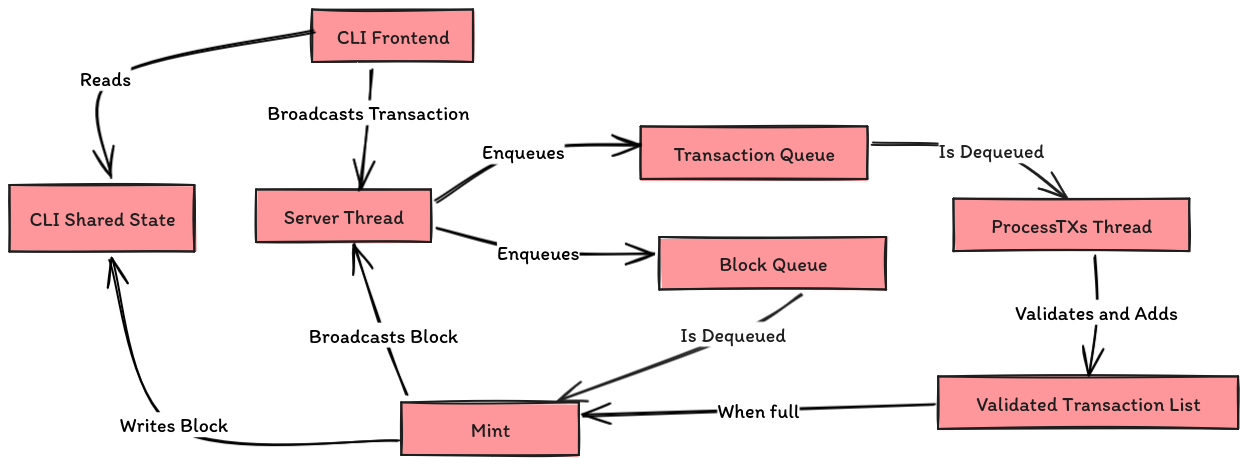
\includegraphics[width=\textwidth]{app-diagram.png}
    \caption{Διάγραμμα Εφαρμογής}
    \label{fig:app-diagram}
\end{figure}

\clearpage
\part{Πειράματα}

Ανά πείραμα αξιολογούνται, αφενός τα πιο χρονοβόρα κομμάτια του κώδικα, όπως
υποδεικνύει το \eng{profiling} καθενός κόμβου κατά την εκτέλεση του πειράματος,
αφετέρου οι συναρτήσεις \eng{mint}, \eng{validateTransaction} και
\eng{processTXs}, οι οποίες συνιστούν την λογική λειτουργίας των κόμβων του
συστήματος. Επίσης, εκτιμάται η ρυθμαπόδοση του συστήματος και το μέσο
\eng{block time}.

\section{Πειραματική Διάταξη}

Απουσία ικανοποιητικής υποδομής κατανεμημένων υπολογιστών, τα πειράματα εκτελέστηκαν
χρησιμοποιώντας \eng{Docker Containers}, τα οποία οδηγήθηκαν καταλλήλως από 
\eng{Bash Scripts}. Τα \eng{containers} χτίστηκαν ως εξής:

\selectlanguage{english}
\lstinputlisting[label={lst:dockerfile}, caption=Dockerfile, language=bash]{../Dockerfile}
\selectlanguage{greek}

και το \eng{script} που οδηγεί τα \eng{containers}:

\selectlanguage{english}
\lstinputlisting[label={lst:docker-driver}, caption=run-docker-experiments.sh, language=bash,
xleftmargin=.1\textwidth]{../run-docker-experiments.sh}
\selectlanguage{greek}



\section{Απόδοση του συστήματος}

Σημειώνεται ότι το ποσοστό του χρόνου εκτέλεσης των σημείων που υποδεικνύει το
\eng{profiling} δεν είναι κληρονομημένο, δηλαδή δεν εμπεριέχονται στο ποσοστό
οι χρόνοι εκτέλεσης των συναρτήσεων που καλούνται από τις συναρτήσεις που
εμφανίζονται στο \eng{profiling}.

\subsection{Χρονοβόρα τμήματα του κώδικα}

Στο πείραμα για την αξιολόγηση της ρυθμαπόδοσης του συστήματος, στήνεται ένα
δίκτυο 5 κόμβων, καθένας εκ των οποίων εκτελεί 1 \eng{staking}, με \eng{stake
10 BCC} συναλλαγή και 50 συναλλαγές (συγκεκριμένα αποστολές μηνυμάτων) προς
τους άλλους κόμβους. Η ταχύτητα αποστολής συναλλαγών είναι ίδια μεταξύ των
κόμβων, ίση με $2\frac{txs}{s}$ και παραμένει σταθερή μεταξύ όλων των
πειραμάτων.

Το πρώτο πράγμα που φαίνεται στο σχήμα \ref{fig:throughput-cost-centers} είναι
ότι το μακράν πιο χρονοβόρο μέρος του κώδικα είναι η συνάρτηση
\eng{modular\_exponentiation} που χρησιμοποιείται γενικά για την κρυπτογράφηση
/ αποκρυπτογράφηση και υπογραφή / επαλήθευση μηνυμάτων. Συγκεκριμένα, φαίνεται
να λαμβάνει περίπου το 45\% του συνολικού χρόνου υπολογισμού\footnote{Ο
\eng{profiler} της \eng{Haskell} μετράει \emph{\eng{CPU time}} όχι
\emph{\eng{blocking time}}} του προγράμματος.

\graphicspath{{../experiments/profiled\_outputs/docker/throughput/}}

\begin{figure}[ht]
    \centering
    \begin{subfigure}{\textwidth}
        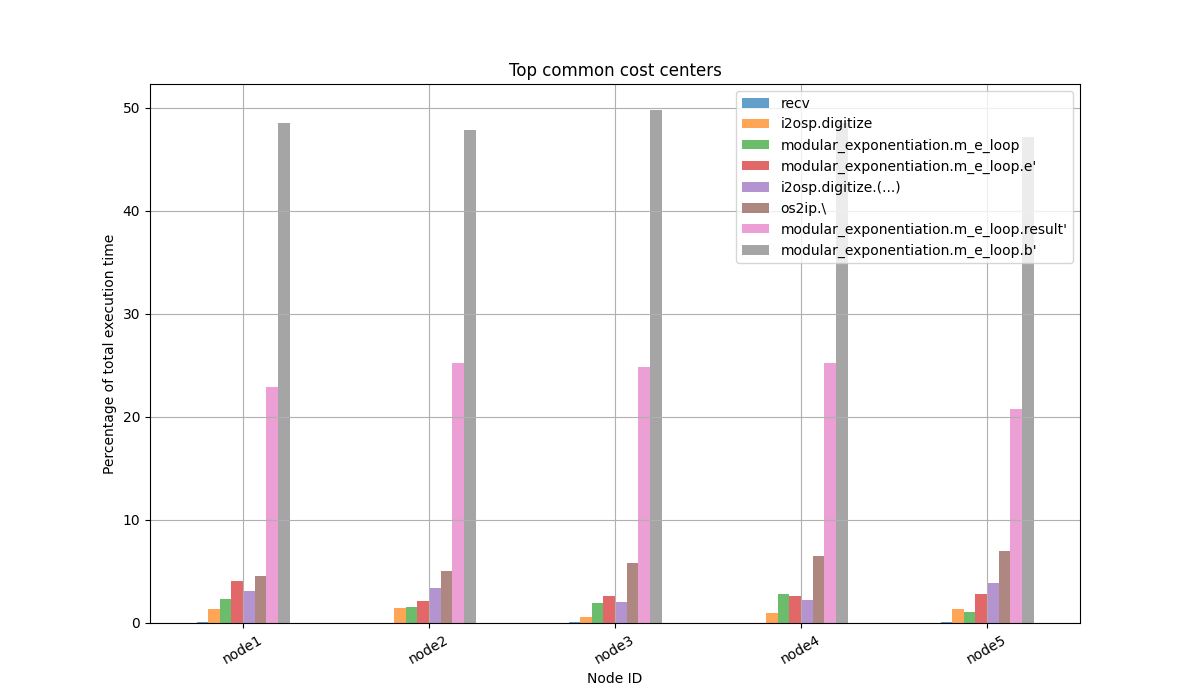
\includegraphics[width=\textwidth]{./capacity5/cost-centers-capacity5.png}
        \caption{\eng{capacity=5}}
    \end{subfigure}
\end{figure}
\begin{figure}[ht]
    \ContinuedFloat
    \begin{subfigure}{\textwidth}
        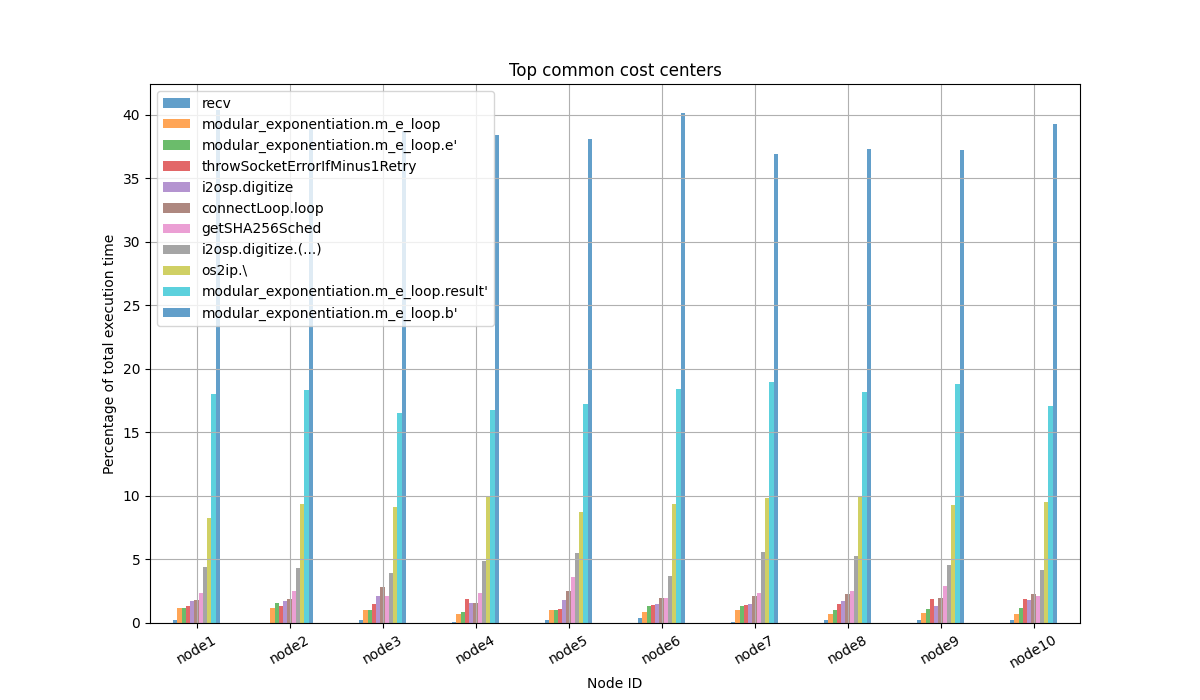
\includegraphics[width=\textwidth]{./capacity10/cost-centers-capacity10.png}
        \caption{\eng{capacity=10}}
    \end{subfigure}
    \begin{subfigure}{\textwidth}
        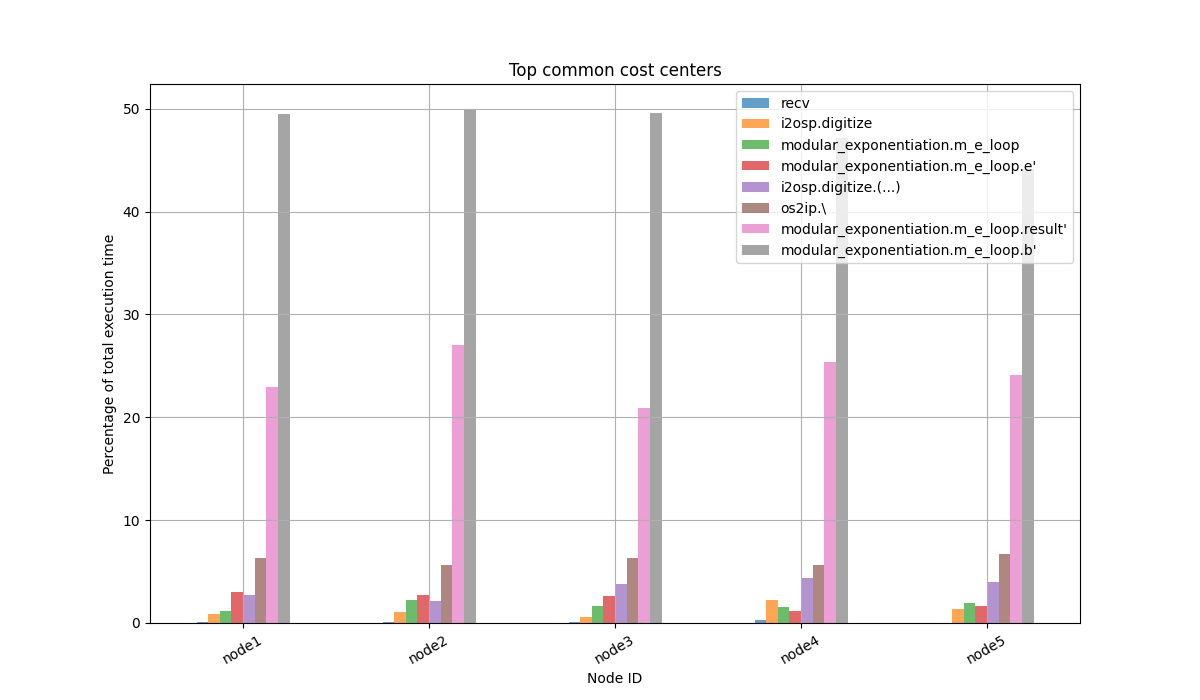
\includegraphics[width=\textwidth]{./capacity20/cost-centers-capacity20.png}
        \caption{\eng{capacity=20}}
    \end{subfigure}
    \caption{Τα πιο χρονοβόρα κομμάτια του κώδικα}
    \label{fig:throughput-cost-centers}
\end{figure}
\FloatBarrier

\subsection{Συναρτήσεις του συστήματος}

Σχετικά με τις \eng{top level} συναρτήσεις του συστήματος, παρατηρείται ότι, με
κάποιες μικρές διακυμάνσεις, η \eng{processTXs} καταναλώνει 9-10\% του
συνολικού \eng{CPU time}, η \eng{mint} 1-3\% και η \eng{validateTransaction}
5-9\%, με μέσο όρο περίπου 6.5\%. 

\begin{figure}[ht]
    \centering
    \begin{subfigure}{\textwidth}
        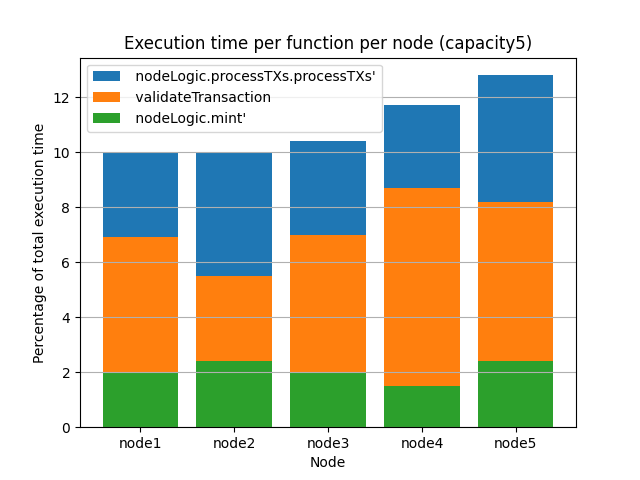
\includegraphics[width=\textwidth]{./capacity5/times_of_function_per_node_capacity5.png}
        \caption{Ρυθμαπόδοση \eng{capacity=5}}
    \end{subfigure}
\end{figure}
\begin{figure}[ht]
    \ContinuedFloat
    \begin{subfigure}{\textwidth}
        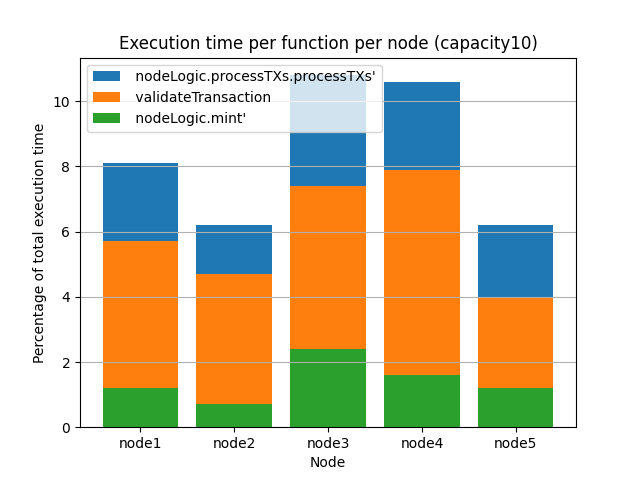
\includegraphics[width=\textwidth]{./capacity10/times_of_function_per_node_capacity10.png}
        \caption{Ρυθμαπόδοση \eng{capacity=10}}
    \end{subfigure}
    \begin{subfigure}{\textwidth}
        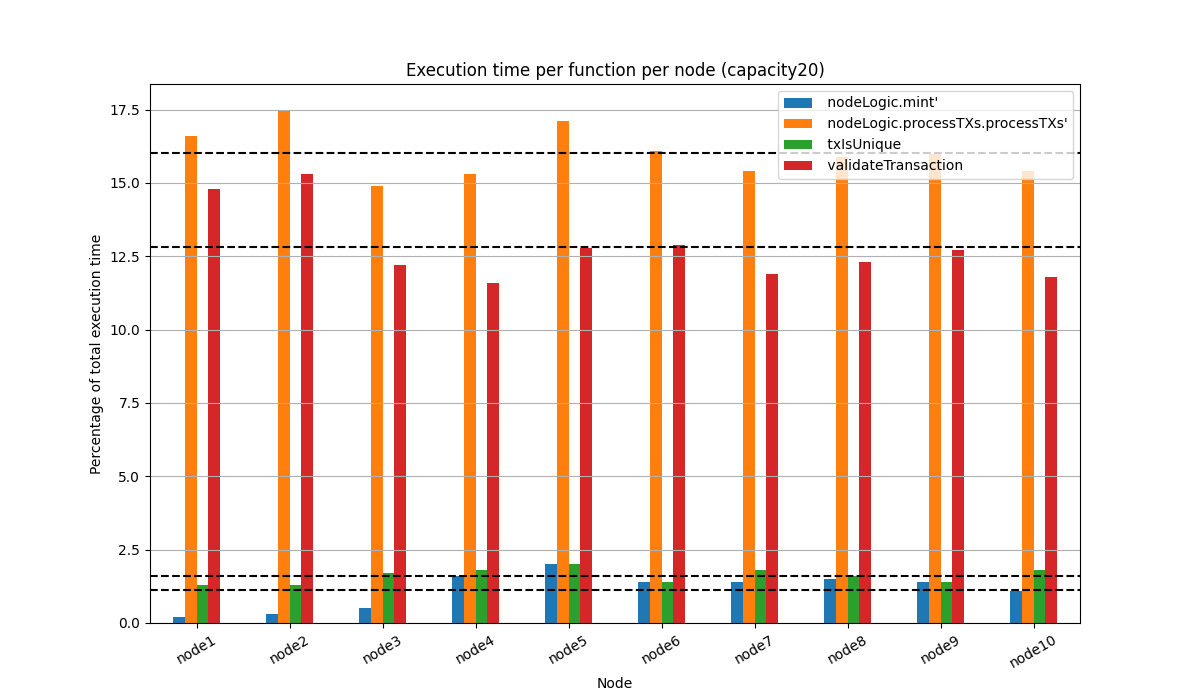
\includegraphics[width=\textwidth]{./capacity20/times_of_function_per_node_capacity20.png}
        \caption{Ρυθμαπόδοση \eng{capacity=20}}
    \end{subfigure}
    \caption{Ποσοστό χρόνου επί του συνολικού χρόνου εκτέλεσης που λαμβάνει η κάθε συνάρτηση}
\end{figure}
\FloatBarrier

Στον πίνακα \ref{tab:throughput-funcs} παρουσιάζονται ορισμένα στατιστικά
σχετικά με τις συναρτήσεις \eng{processTXs}, \eng{validateTransaction},
\eng{txIsUnique} και \eng{mint}. Το πιο σημαντικό να παρατηρηθεί είναι ότι, για
κάθε κόμβο, οι κλήσεις στην συνάρτηση \eng{validateTransaction} είναι ακριβώς
τόσες όσες και οι συναλλαγές που αποστέλλονται από όλους τους κόμβους $\left(5
+ 5 \times 50 = 255 \right)$. Επίσης, $\#mint + \#validateTransaction =
\#processTXs$ \footnote{Η -1 διαφορά είναι επειδή έγινε η τελευταία κλήση και τα
προγράμματα έλαβαν σήμα τερματισμού}. Παρ'ότι φαίνεται σαν να επικυρώθηκαν όλες
οι συναλλαγές, αυτό δεν ισχύει. Στην πραγματικότητα, επειδή οι κόμβοι δεν 
παραλαμβάνουν κατ' ανάγκην τις συναλλαγές με την σειρά αποστολή τους, είναι πιθανό
κάποιος \eng{validator} να ακυρώσει κάποια συναλλαγή η οποία με διαφορετική σειρά
θα είχε επιβεβαιωθεί. Για αυτόν τον λόγο φαίνεται ότι ένα υποσύνολο των
συναλλαγών εξετάζεται για την μοναδικότητά τους από την συνάρτηση
\eng{txIsUnique}. Έτσι αιτιολογείται και το γεγονός ότι το \eng{blockchain}
έχει μήκος μικρότερο από το μέγιστο δυνατό του δεδομένων των συναλλαγών.
Παραδείγματος χάριν, για \eng{capacity 5} έχει μήκος $41 = \frac{207}{5} <
\frac{255}{5} = 51$.

\DTLloaddb{th-calls1}{../experiments/profiled_outputs/docker/throughput/capacity5/rawinfo.csv}
\DTLloaddb{th-calls2}{../experiments/profiled_outputs/docker/throughput/capacity10/rawinfo.csv}
\DTLloaddb{th-calls3}{../experiments/profiled_outputs/docker/throughput/capacity20/rawinfo.csv}

\begin{table}[ht]
    \caption{Στατιστικά συναρτήσεων ανά κόμβο} 
    \label{tab:throughput-funcs}
    \begin{subtable}{\textwidth}
        \centering
        \caption{\eng{capacity=5}}
        \label{tab:throughput-funcs-1}
        \selectlanguage{english}
        \DTLdisplaydb[Module,Source,Number,TimeInd,MemInd,MemInh]{th-calls1}
        \selectlanguage{greek}
    \end{subtable}
\end{table}

Όπως φαίνεται από τον πίνακα, λοιπόν, για τον υπολογισμό του \eng{block time} και
της ρυθμαπόδοσης λαμβάνονται υπόψιν τόσα μπλοκς όσα και οι κλήσεις στην συνάρτηση
\eng{mint} και τόσες συναλλαγές όσες τα μπλοκς επί την εκάστοτε χωρητικότητα.

\begin{equation}
    \begin{gathered}
        \text{Χωρητικότητα = 5} \Rightarrow \text{Μπλοκς} = 45 \text{ και } \text{Συναλλαγές} = 225 \\
        \text{Χωρητικότητα = 10} \Rightarrow \text{Μπλοκς} = 22 \text{ και } \text{Συναλλαγές} = 220 \\
        \text{Χωρητικότητα = 20} \Rightarrow \text{Μπλοκς} = 11 \text{ και } \text{Συναλλαγές} = 220 \\
    \end{gathered}
\end{equation}

\begin{table}[ht]
    \ContinuedFloat
    \begin{subtable}{0.45\textwidth}
        \centering
        \caption{\eng{capacity=10}}
        \label{tab:throughput-funcs-2}
        \selectlanguage{english}
        \DTLdisplaydb[Module,Source,Number,TimeInd,MemInd,MemInh]{th-calls2}
        \selectlanguage{greek}
    \end{subtable}
    \hfill
    \begin{subtable}{0.45\textwidth}
        \centering
        \caption{\eng{capacity=20}}
        \label{tab:throughput-funcs-3}
        \selectlanguage{english}
        \DTLdisplaydb[Module,Source,Number,TimeInd,MemInd,MemInh,Node,Function]{th-calls3}
        \selectlanguage{greek}
    \end{subtable}
\end{table}
\FloatBarrier

\subsection{Ρυθμαπόδοση και \eng{Block time}}

Το \eng{block time} μπορεί να υπολογιστεί λαμβάνοντας τον μέσο όρο των
διαφορών των \eng{time stamps} διαδοχικών \eng{blocks}. Στο σχήμα
\ref{fig:throughput-blocktimes} φαίνονται οι χρόνοι δημιουργίας \eng{block} όπως
υπολογίστηκαν από κάθε κόμβο. Παρατηρείται ότι δεν είναι πάντοτε ίσοι μεταξύ
των κόμβων. Αυτό συμβαίνει γιατί, κατά τον τερματισμό του πειράματος, δεν έχουν
φτάσει κατ'ανάγκην όλοι οι κόμβοι στο ίδιο σημείο της αλυσίδας και για αυτόν τον
λόγο διαφοροποιείται η μέτρησή τους. Εδώ λαμβάνεται υπόψιν το μέγιστο μήκος της
αλυσίδας μεταξύ των κόμβων.

\begin{figure}[ht]
    \centering
    \selectlanguage{english}
    \begin{varwidth}{\linewidth}
        \verbatiminput{../experiments/profiled_outputs/docker_harmonic/throughput/blocktimes.txt}
    \end{varwidth}
    \selectlanguage{greek}
    \caption{Μέσος χρόνος δημιουργίας \eng{block} (\eng{ms})}
    \label{fig:throughput-blocktimes}
\end{figure}

Από τον χρόνο αυτόν μπορούν να μετρηθούν και οι εξυπηρετούμενες συναλλαγές ανά δευτερόλεπτο.
Συγκεκριμένα, μία συναλλαγή εξυπηρετείται όταν επικυρωθεί, δηλαδή όταν καταγραφεί στην αλυσίδα.
Άρα, για κάθε \eng{capacity} έχουμε:

\begin{equation}
    \begin{gathered}
        \text{Ρυθμαπόδοση} = \frac{\text{Συναλλαγές}}{\text{Χρόνος}} = \frac{\text{Συναλλαγές}}{\text{Μπλοκ}}\cdot \frac{\text{Μπλοκ}}{\text{Χρόνος}} \Leftrightarrow \\
        \text{Ρυθμαπόδοση} = \frac{\frac{\text{Συναλλαγές}}{\text{Μπλοκ}} }{\text{Μέσος χρόνος δημιουργίας μπλοκ}} = \frac{\text{Χωρητικότητα}}{\text{Μέσος χρόνος δημιουργίας μπλοκ}} \Rightarrow \\
    \boxed{
        \begin{gathered}
            \text{Ρυθμαπόδοση}_{capacity=5} = \frac{5}{0,024} = 208,333\text{} \frac{txs}{s}\\
            \text{Ρυθμαπόδοση}_{capacity=10} = \frac{10}{0,0626} = 159,744\text{} \frac{txs}{s}\\
            \text{Ρυθμαπόδοση}_{capacity=20} = \frac{20}{0,121} = 165,289\text{} \frac{txs}{s}\\
        \end{gathered}
    }
    \end{gathered}
\end{equation}

% Χρησιμοποιώντας τα στατιστικά από το \eng{profiling} καθενός κόμβου
% μπορούν να εκτιμηθούν η ρυθμαπόδοση και το μέσο \eng{block time}.
% 
% \begin{figure}[ht]
%     \begin{subfigure}{\textwidth}
%         \centering
%         \caption{\eng{capacity=5}}
%         \label{fig:throughput-times-5}
%         \selectlanguage{english}
%         \begin{varwidth}{\linewidth}
%             \verbatiminput{../experiments/profiled_outputs/docker/throughput/capacity5/final.csv}
%         \end{varwidth}
%         \selectlanguage{greek}
%     \end{subfigure}
%     \begin{subfigure}{\textwidth}
%         \centering
%         \caption{\eng{capacity=10}}
%         \label{fig:throughput-times-10}
%         \selectlanguage{english}
%         \begin{varwidth}{\linewidth}
%             \verbatiminput{../experiments/profiled_outputs/docker/throughput/capacity10/final.csv}
%         \end{varwidth}
%         \selectlanguage{greek}
%     \end{subfigure}
%     \begin{subfigure}{\textwidth}
%         \centering
%         \caption{\eng{capacity=20}}
%         \label{fig:throughput-times-20}
%         \selectlanguage{english}
%         \begin{varwidth}{\linewidth}
%             \verbatiminput{../experiments/profiled_outputs/docker/throughput/capacity20/final.csv}
%         \end{varwidth}
%         \selectlanguage{greek}
%     \end{subfigure}
%     \caption{Χρόνοι εκτέλεσης κόμβων}
%     \label{fig:throughput-times}
% \end{figure}
% \FloatBarrier

\clearpage
\section{Κλιμακωσιμότητα του συστήματος}

Στο πείραμα κλιμακωσιμότητας, το δίκτυο εκκινείται με 10 κόμβους, καθένας εκ
των οποίων εκτελεί 1 \eng{staking} συναλλαγή, με \eng{stake 10 BCC} και 100
συναλλαγές (συγκεκριμένα αποστολές μηνυμάτων) προς τους άλλους κόμβους. Σκοπός
είναι να εξεταστεί η κλιμάκωση του συστήματος ως προς το πλήθος των
συμμετεχόντων κόμβων.

\subsection{Χρονοβόρα τμήματα του κώδικα}

Στα γραφήματα \ref{fig:scalability-cost-centers} φαίνονται τα πιο χρονοβόρα
κομμάτια του κώδικα για κάθε πείραμα κλιμακωσιμότητας. Φαίνεται ότι αυτά είναι
τα ίδια με τα πιο χρονοβόρα κομμάτια του κώδικα για το πείραμα ρυθμαπόδοσης, με
την συνάρτηση \eng{modular\_exponentiation} να καταλαμβάνει πάλι περίπου το
45\% του συνολικού \eng{CPU time} του προγράμματος.

\graphicspath{{../experiments/profiled\_outputs/docker/scalability/}}

\begin{figure}[ht]
    \centering
    \begin{subfigure}{\textwidth}
        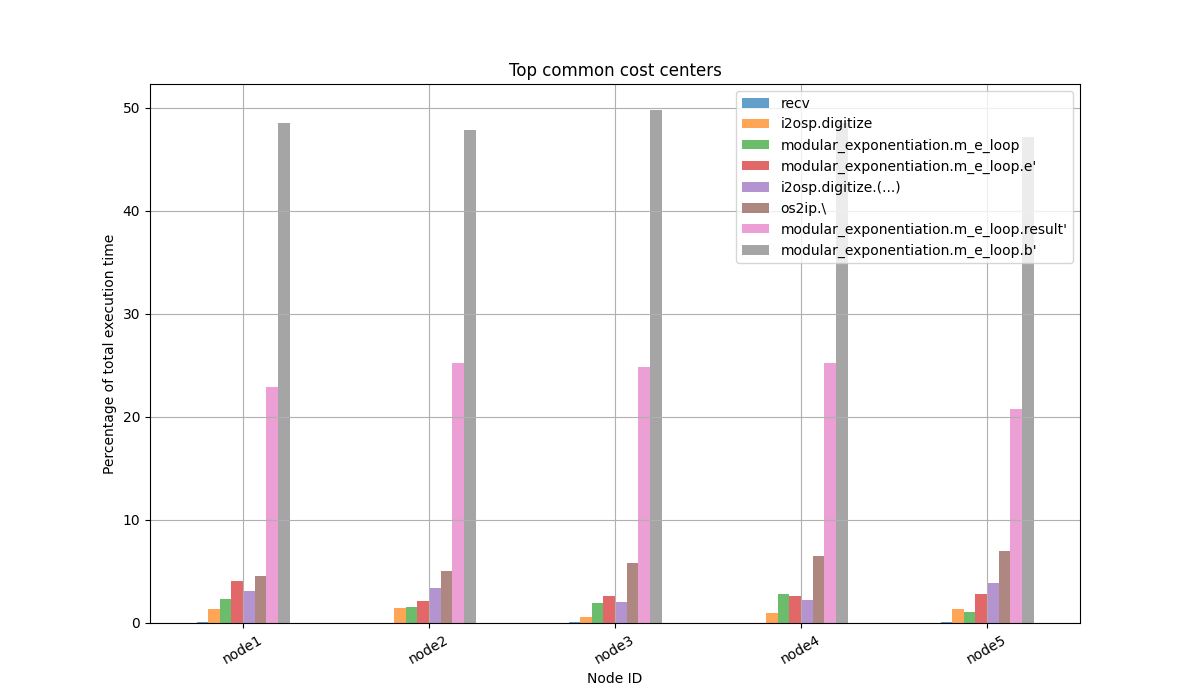
\includegraphics[width=\textwidth]{./capacity5/cost-centers-capacity5.png}
        \caption{\eng{capacity=5}}
    \end{subfigure}
\end{figure}
\begin{figure}[ht]
    \ContinuedFloat
    \begin{subfigure}{\textwidth}
        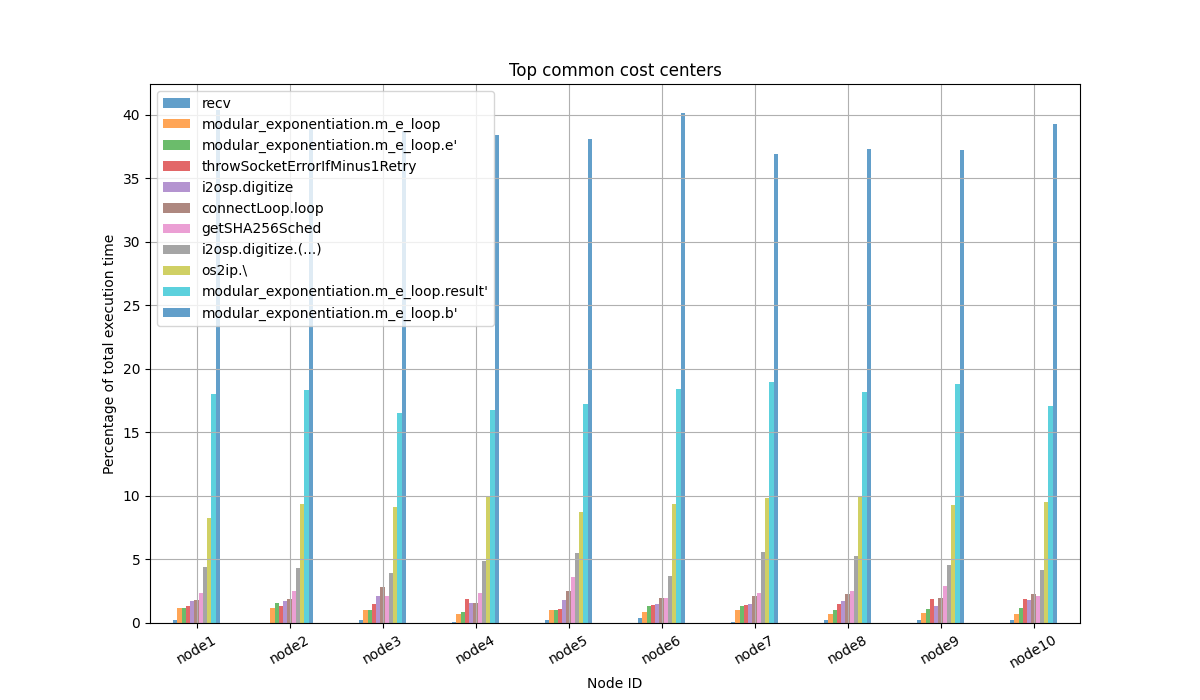
\includegraphics[width=\textwidth]{./capacity10/cost-centers-capacity10.png}
        \caption{\eng{capacity=10}}
    \end{subfigure}
    \begin{subfigure}{\textwidth}
        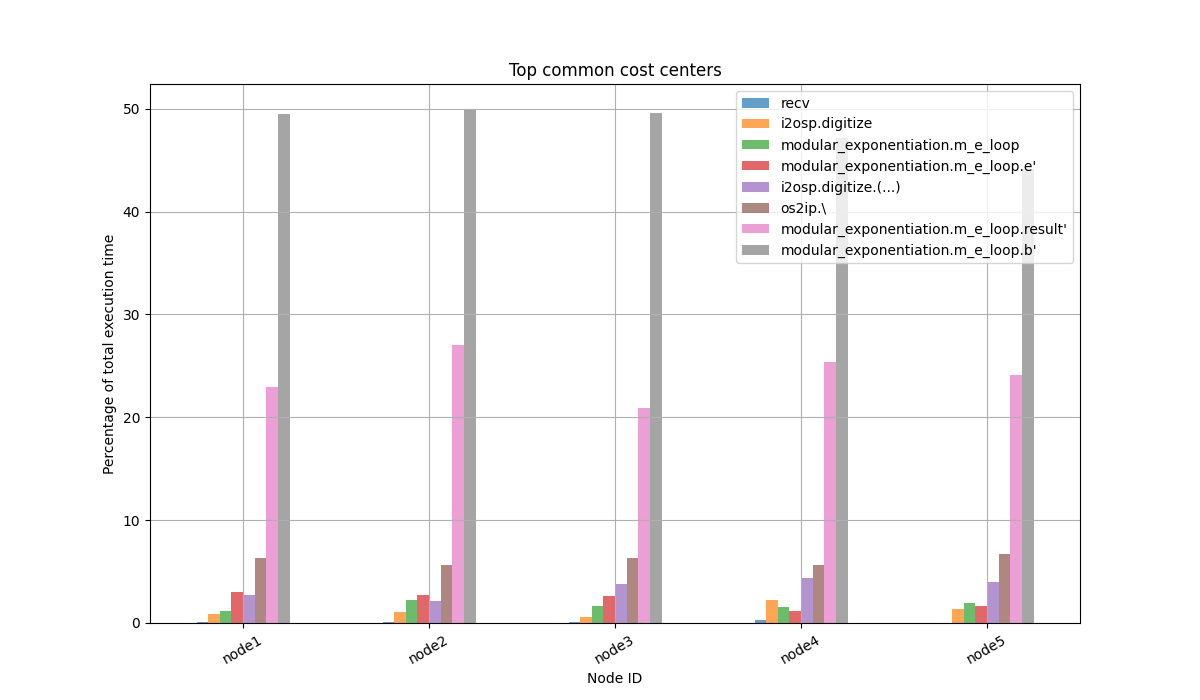
\includegraphics[width=\textwidth]{./capacity20/cost-centers-capacity20.png}
        \caption{\eng{capacity=20}}
    \end{subfigure}
    \caption{Τα πιο χρονοβόρα κομμάτια του κώδικα}
    \label{fig:scalability-cost-centers}
\end{figure}
\FloatBarrier

\subsection{Συναρτήσεις του συστήματος}

Στα γραφήματα \ref{fig:scalability-funcs} παρατηρείται ότι οι συναρτήσεις
καταλαμβάνουν περίπου το ίδιο ποσοστό χρόνου εκτέλεσης με το προηγούμενο
πείραμα.

\begin{figure}[ht]
    \centering
    \begin{subfigure}{\textwidth}
        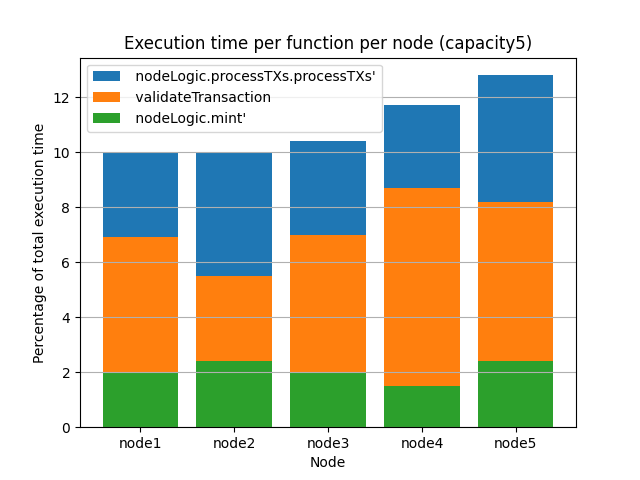
\includegraphics[width=\textwidth]{./capacity5/times_of_function_per_node_capacity5.png}
        \caption{\eng{capacity=5}}
        \label{fig:scalability-funcs-5}
    \end{subfigure}
\end{figure}
\begin{figure}[ht]
    \ContinuedFloat
    \begin{subfigure}{\textwidth}
        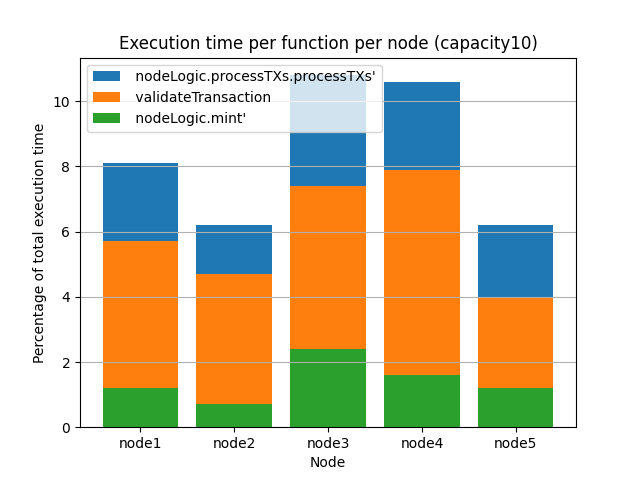
\includegraphics[width=\textwidth]{./capacity10/times_of_function_per_node_capacity10.png}
        \caption{\eng{capacity=10}}
        \label{fig:scalability-funcs-10}
    \end{subfigure}
    \centering
    \begin{subfigure}{\textwidth}
        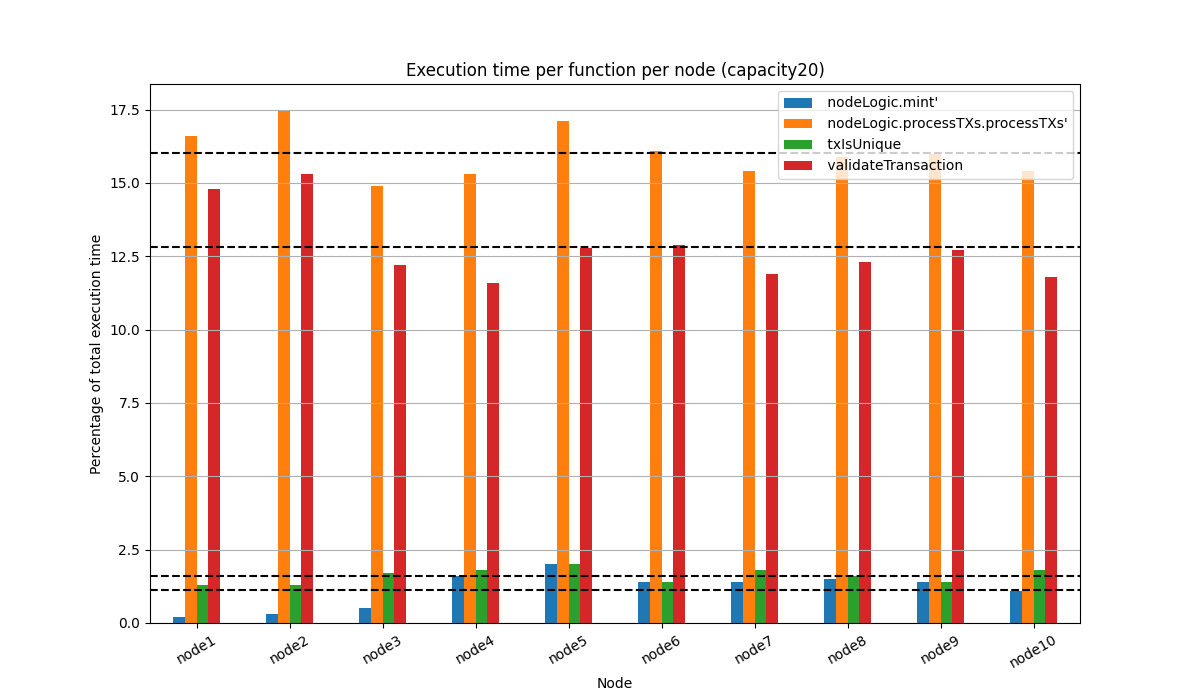
\includegraphics[width=\textwidth]{./capacity20/times_of_function_per_node_capacity20.png}
        \caption{\eng{capacity=20}}
        \label{fig:scalability-funcs-20}
    \end{subfigure}
    \caption{Ποσοστό χρόνου επί του συνολικού χρόνου εκτέλεσης που λαμβάνει η κάθε συνάρτηση}
    \label{fig:scalability-funcs}
\end{figure}
\FloatBarrier

\DTLloaddb{sc-calls1}{../experiments/profiled_outputs/docker/scalability/capacity5/rawinfo.csv}
\DTLloaddb{sc-calls2}{../experiments/profiled_outputs/docker/scalability/capacity10/rawinfo.csv}
\DTLloaddb{sc-calls3}{../experiments/profiled_outputs/docker/scalability/capacity20/rawinfo.csv}

Στον πίνακα \ref{tab:scalability-funcs-1} φαίνονται οι κλήσεις ενδιαφέροντος
των κόμβων. Παρατηρώντας το πλήθος των κλήσεων ανά συνάρτηση, διαπιστώνεται ότι
οι κόμβοι δεν προλαβαίνουν να επικυρώσουν όλες τις συναλλαγές που λαμβάνουν.
Αυτό οφείλεται, αφενός στον μεγαλύτερο όγκο συναλλαγών $10 + 10 \times 100 =
1010$ ο οποίος είναι $\approx 4$ φορές μεγαλύτερος από προηγουμένως, και
αφετέρου στην μικρή χωρητικότητα του \eng{block}, το οποίο σημαίνει ότι οι
κόμβοι πρέπει συχνά να καλούν την χρονοβόρα συνάρτηση \eng{mint} και να
διακόπτουν την διαδικασία επικύρωσης.

Επίσης, παρατηρείται ότι οι κόμβοι 7-8 έχουν μείνει πολύ πίσω σε σχέση
με τους υπόλοιπους κόμβους. Αυτό είναι μάλλον συνέπεια της πειραματικής
διάταξης, αφού όλοι οι κόμβοι τρέχουν στο ίδιο μηχάνημα.

\begin{table}[ht]
    \caption{Στατιστικά συναρτήσεων ανά κόμβο}
    \label{tab:scalability-funcs}
    \begin{subtable}{\textwidth}
        \centering
        \caption{\eng{capacity=5}}
        \label{tab:scalability-funcs-1}
        \selectlanguage{english}
        \DTLdisplaydb[Module,Source,Number,TimeInd,MemInd,MemInh]{sc-calls1}
        \selectlanguage{greek}
    \end{subtable}
\end{table}

Αντιθέτως, στους πίνακες \ref{tab:scalability-funcs-2} και \ref{tab:scalability-funcs-3}
φαίνεται από τις κλήσεις των συναρτήσεων ότι έχουν επικυρωθεί όλες οι συναλλαγές
και έχουν παραχθεί τα αντίστοιχα \eng{blocks}. Η μεγαλύτερη χωρητικότητα των
\eng{blocks} επιτρέπει στους κόμβους μεγαλύτερα χρονικά παράθυρα για την
επικύρωση των συναλλαγών και η διακοπή για την παραγωγή των \eng{blocks} δεν
καθυστερεί την εξέλιξη του δικτύου.

\begin{table}[ht]
    \ContinuedFloat
    \begin{subtable}{0.45\textwidth}
        \centering
        \caption{\eng{capacity=10}}
        \label{tab:scalability-funcs-2}
        \selectlanguage{english}
        \DTLdisplaydb[Module,Source,Number,TimeInd,MemInd,MemInh]{sc-calls2}
        \selectlanguage{greek}
    \end{subtable}
    \hfill
    \begin{subtable}{0.45\textwidth}
        \centering
        \caption{\eng{capacity=20}}
        \label{tab:scalability-funcs-3}
        \selectlanguage{english}
        \DTLdisplaydb[Module,Source,Number,TimeInd,MemInd,MemInh,Node,Function]{sc-calls3}
        \selectlanguage{greek}
    \end{subtable}
\end{table}
\FloatBarrier

Για την μέτρηση του \eng{block time} και της ρυθμαπόδοσης του συστήματος, λαμβάνονται
υπόψιν τόσα μπλοκ όσα και οι κλήσεις στην συνάρτηση \eng{mint} και τόσες συναλλαγές
όσα τα μπλοκς επί την εκάστοτε χωρητικότητα.

\begin{equation}
    \begin{gathered}
        \text{Χωρητικότητα = 5} \Rightarrow \text{Μπλοκς} = 100 \text{ και } \text{Συναλλαγές} = 500 \\
        \text{Χωρητικότητα = 10} \Rightarrow \text{Μπλοκς} = 50 \text{ και } \text{Συναλλαγές} = 500 \\
        \text{Χωρητικότητα = 20} \Rightarrow \text{Μπλοκς} = 25 \text{ και } \text{Συναλλαγές} = 500 \\
    \end{gathered}
\end{equation}

\clearpage
\subsection{Ρυθμαπόδοση και \eng{Block time}}

Στο σχήμα \ref{fig:scalability-blocktimes} φαίνονται οι μέσοι
χρόνοι\footnote{Αρμονικός μέσος.} δημιουργίας \eng{block} όπως υπολογίστηκαν
από κάθε κόμβο\footnote{Οι χρόνοι αυτοί λήφθηκαν χωρίς \eng{profiling}
ενεργοποιημένο, ώστε να μην υπάρχουν παρεμβολές. Τα προηγούμενα στοιχεία
\eng{profiling}, δηλαδή το πλήθος κλήσεων σε διάφορες συναρτήσεις,
παρουσιάστηκαν ως ενδεικτικά για την συμπεριφορά των κόμβων.}.

\begin{figure}[ht]
    \centering
    \selectlanguage{english}
    \begin{varwidth}{\linewidth}
        \verbatiminput{../experiments/profiled_outputs/docker_harmonic/scalability/blocktimes.txt}
    \end{varwidth}
    \selectlanguage{greek}
    \caption{Μέσος χρόνος δημιουργίας \eng{block} (\eng{ms})}
    \label{fig:scalability-blocktimes}
\end{figure}

Πάλι, από τους χρόνους αυτούς μπορούν να μετρηθούν και οι εξυπηρετούμενες
συναλλαγές ανά δευτερόλεπτο. Για κάθε \eng{capacity} έχουμε:

\begin{equation}
    \begin{gathered}
        \text{Ρυθμαπόδοση} = \frac{\text{Συναλλαγές}}{\text{Χρόνος}} = \frac{\text{Συναλλαγές}}{\text{Μπλοκ}}\cdot \frac{\text{Μπλοκ}}{\text{Χρόνος}} \Leftrightarrow \\
        \\
        \text{Ρυθμαπόδοση} = \frac{\frac{\text{Συναλλαγές}}{\text{Μπλοκ}} }{\text{Μέσος χρόνος δημιουργίας μπλοκ}} = \frac{\text{Χωρητικότητα}}{\text{Μέσος χρόνος δημιουργίας μπλοκ}} \Rightarrow \\
    \\
    \boxed{
        \begin{gathered}
            \text{Ρυθμαπόδοση}_{capacity=5} = \frac{5}{0,0404} = 123,639 \text{} \frac{txs}{s}\\
            \text{Ρυθμαπόδοση}_{capacity=10} = \frac{10}{0.1097} = 91,157 \text{} \frac{txs}{s}\\
            \text{Ρυθμαπόδοση}_{capacity=20} = \frac{20}{0.1095} = 182,648 \text{} \frac{txs}{s}\\
        \end{gathered}
    }
    \end{gathered}
\end{equation}

Οι μετρήσεις από τα πειράματα συνοψίζονται στα γραφήματα \ref{fig:throughput-block-time}.

\begin{figure}
    \begin{subfigure}{\textwidth}
        \centering
        \caption{\eng{Throughput} του συστήματος}
        \label{fig:throughput-per-node}
        \selectlanguage{english}
        \adjustbox{width=0.7\textwidth}{
            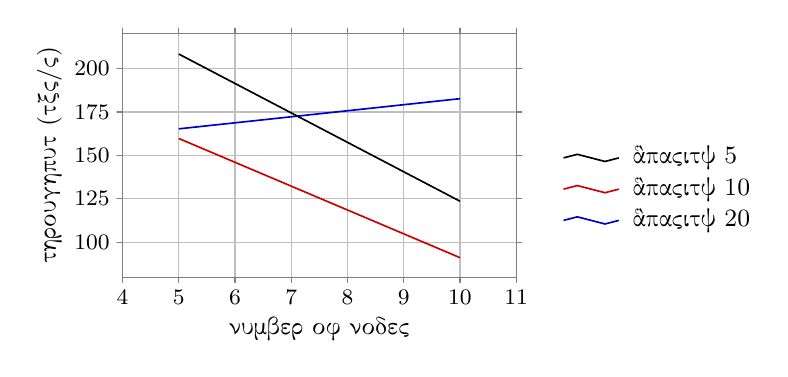
\begin{tikzpicture}
                \datavisualization [scientific axes, all axes={grid},
                                    visualize as line/.list={capacity5, capacity10, capacity20},
                                    x axis={label={number of nodes}, 
                                            min value=4, max value=11},
                                    y axis={label={throughput (txs/s)},
                                            min value=80, max value=220},
                                    capacity5={label in legend={text=Capacity 5}},
                                    capacity10={label in legend={text=Capacity 10}},
                                    capacity20={label in legend={text=Capacity 20}},
                                    legend=east outside, style sheet=strong colors,
                                    ]
                    data [set=capacity5] {
                        x, y
                        5, 208.333
                        10, 123.639
                    }
                    data [set=capacity10] {
                        x, y
                        5, 159.744
                        10, 91.157
                    }
                    data [set=capacity20]{
                        x, y
                        5, 165.289
                        10, 182.648
                    };
            \end{tikzpicture}
        }
        \selectlanguage{greek}
    \end{subfigure}
    \begin{subfigure}{\textwidth}
        \centering
        \caption{Μέσο \eng{block time} του συστήματος}
        \label{fig:block-time-per-node}
        \selectlanguage{english}
        \adjustbox{width=0.7\textwidth}{
            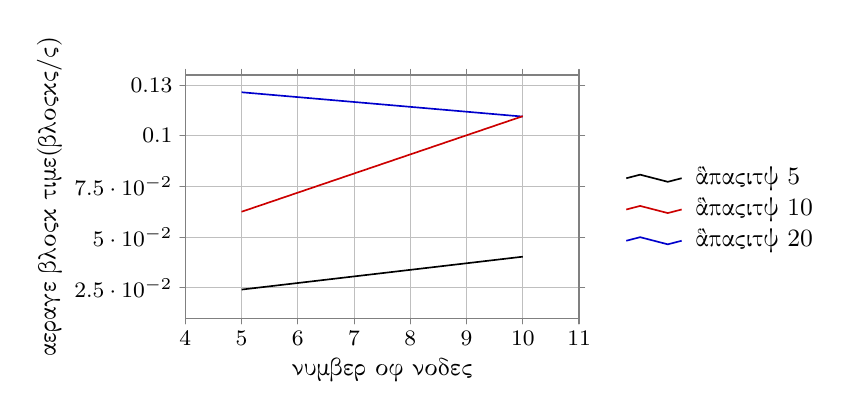
\begin{tikzpicture}
                \datavisualization [
                    scientific axes, all axes={grid},
                    visualize as line/.list={capacity5, capacity10, capacity20},
                    x axis={label={number of nodes}, 
                            min value=4, max value=11},
                    y axis={label={average block time(blocks/s)},
                            min value=0.01, max value=0.13},
                    capacity5={label in legend={text=Capacity 5}},
                    capacity10={label in legend={text=Capacity 10}},
                    capacity20={label in legend={text=Capacity 20}},
                    legend=east outside, style sheet=strong colors,
                ]
                    data [set=capacity5] {
                        x, y
                        5, 0.02418
                        10, 0.0404
                    }
                    data [set=capacity10] {
                        x, y
                        5, 0.06256
                        10, 0.1097
                    }
                    data [set=capacity20]{
                        x, y
                        5, 0.1215
                        10, 0.1095
                    };
            \end{tikzpicture}
        }
        \selectlanguage{greek}
    \end{subfigure}
    \caption{Ρυθμαπόδοση και μέσος \eng{block time} του συστήματος}
    \label{fig:throughput-block-time}
\end{figure}
\FloatBarrier

Στα γραφήματα \ref{fig:throughput-per-node} και \ref{fig:block-time-per-node}
φαίνεται η ρυθμαπόδοση και το μέσο \eng{block time} του συστήματος μεταξύ των
πειραμάτων, από 5 έως 10 κόμβους, για κάθε χωρητικότητα. Φαίνεται, ότι το
πλήθος των εξυπηρετούμενων συναλλαγών ανά μονάδα χρόνου αυξάνεται με τον αριθμό
των κόμβων για την χωρητικότητα 20, αλλά για την 5 και 10 ελαττώνεται. Ο δε
μέσος χρόνος δημιουργίας \eng{block} μειώνεται με τον αριθμό των κόμβων για την
χωρητικότητα 20, αλλά για την 5 και 10 έχει αύξουσα τάση. Αυτό δείχνει ότι το
δίκτυο μπορεί να κλιμακώνει με τον αριθμό των κόμβων για χωρητικότητα 20.

\clearpage
\section{Δικαιοσύνη}

Στο πείραμα δικαιοσύνης, το δίκτυο εκκινείται με 5 κόμβους και ο υπ'αριθμόν 1
από αυτούς κάνει \eng{stake 100 BCC}, ενώ οι υπόλοιποι κάνουν \eng{stake 10 BCC}.

\graphicspath{{../experiments/profiled\_outputs/docker/fairness/}}
\begin{figure}[ht]
    \centering
    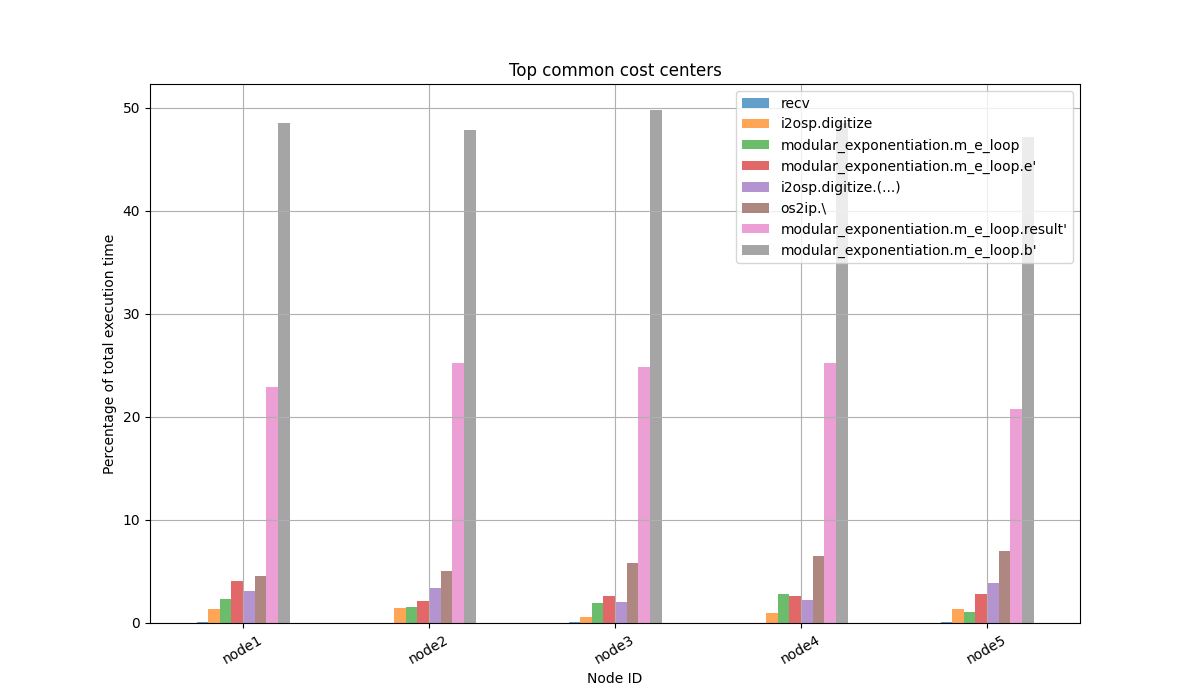
\includegraphics[width=\textwidth]{./capacity5/cost-centers-capacity5.png}
    \caption{Τα πιο χρονοβόρα κομμάτια του κώδικα \eng{capacity=5}}
    \label{fig:fairness-cost-centers}
\end{figure}

Στον πίνακα \ref{tab:fairness-funcs} φαίνονται οι κλήσεις μερικών συναρτήσεων
ενδιαφέροντος. Φαίνεται ότι τα πλήθη όλων των κλήσεων είναι ίδια ανά κόμβο,
πράγμα που σημαίνει ότι οι κόμβοι εκτελούν τις ίδιες λειτουργίες με την ίδια
συχνότητα. Παρ'όλα αυτά, ο κόμβος με το μεγαλύτερο \eng{stake} καταναλώνει πολύ
περισσότερο χρόνο στην συνάρτηση \eng{mint'} σε σχέση με τους υπόλοιπους
κόμβους, όπως φαίνεται και στο σχήμα \ref{fig:fairness-funcs}.

\DTLloaddb{fairness-calls}{../experiments/profiled_outputs/docker/fairness/capacity5/rawinfo.csv}
\begin{table}[ht]
    \centering
    \caption{Στατιστικά συναρτήσεων ανά κόμβο \eng{capacity=5}}
    \label{tab:fairness-funcs}
    \selectlanguage{english}
    \DTLdisplaydb[Module,Source,Number,TimeInd,MemInd,MemInh]{fairness-calls}
    \selectlanguage{greek}
\end{table}

\begin{figure}[ht]
    \centering
    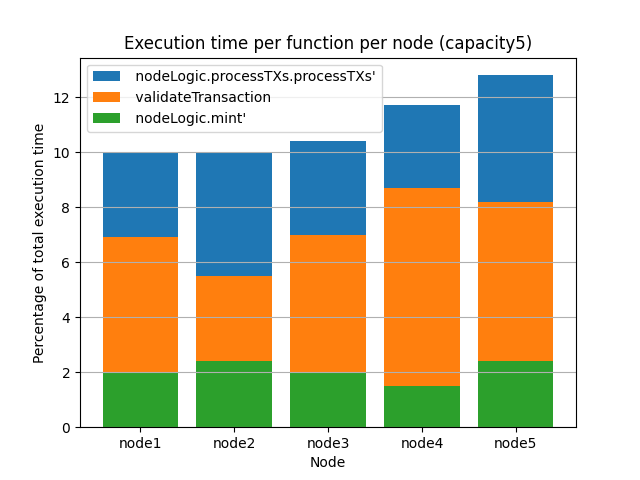
\includegraphics[width=\textwidth]{./capacity5/times_of_function_per_node_capacity5.png}
    \caption{Ποσοστό χρόνου επί του συνολικού χρόνου εκτέλεσης που λαμβάνει η κάθε συνάρτηση \eng{capacity=5}}
    \label{fig:fairness-funcs}
\end{figure}
\FloatBarrier

Στο σχήμα \ref{fig:fairness-funcs} φαίνεται, πράγματι, ότι ο κόμβος με το
μεγαλύτερο \eng{stake} καταναλώνει πολύ περισσότερο χρόνο στην συνάρτηση
\eng{mint'} σε σχέση με τους υπόλοιπους κόμβους, ενδεικτικό του γεγονός ότι
πράγματι αυτός αναλαμβάνει συχνότερα την δημιουργία των νέων \eng{blocks}.
Μάλιστα, επισκοπώντας τα υπόλοιπα των λογαριασμών των κόμβων στο σχήμα
\ref{fig:fairness-balances}, παρατηρεί κανείς ότι όντως τα περισσότερα
νομίσματα συσσωρεύονται στον κόμβο με το μεγαλύτερο \eng{stake}. Συμπεραίνεται,
λοιπόν, ότι σε βάθος χρόνου συσσωρεύονται νομίσματα στον κόμβο με το μεγαλύτερο
\eng{stake}. Θεωρητικά, αυτό σημαίνει ότι ένας κακόβουλος κόμβος θα μπορούσε
να εκμεταλλευτεί το φαινόμενο αυτό και να χειραγωγεί το δίκτυο κατά την
θέλησή του. Επομένως, υπάρχει ανάγκη για έναν μηχανισμό που θα εξασφαλίζει
ότι, παρά την ανισότητα των \eng{stakes}, οι κόμβοι θα έχουν ίσες ευκαιρίες
στην επικύρωση των συναλλαγών και δεν θα επαφίεται η ασφάλεια του δικτύου
σε έναν μόνο κόμβο.

\begin{figure}[h]
    \centering    
    \selectlanguage{english}
    \begin{varwidth}{\linewidth}
        \verbatiminput{../experiments/profiled_outputs/docker/fairness/capacity5/balances.out}
    \end{varwidth}
    \selectlanguage{greek}
    \caption{Υπόλοιπα λογαριασμών κόμβων \eng{capacity=5}}
    \label{fig:fairness-balances}
\end{figure}

\end{document}

